%%%%%%%%%%%%%%%%%%%%%%%%%%%%%%%%%%%%%%%%%%%%%%%%%%%%%%%%%%%%%%%%%%%%%%%%%%%%%%%%
% Template for ASPLOS papers.
%
% History:
% 
% ASPLOS originally used jpaper.cls for submission but required acmart.cls for the
% final camera-ready version. To avoid a change in format, starting ASPLOS 2024 Fall 
% cycle, both the submission and the camera-ready versions started using acmart.cls.
%
%%%%%%%%%%%%%%%%%%%%%%%%%%%%%%%%%%%%%%%%%%%%%%%%%%%%%%%%%%%%%%%%%%%%%%%%%%%%%%%%%%

% use the base acmart.cls version 1.92
% use the sigplan proceeding template with the default 10 pt fonts
% nonacm option removes ACM related text in the submission. 
\documentclass[nonacm,sigplan]{acmart}

% enable page numbers
\settopmatter{printfolios=true}

% make references clickable 
\usepackage[]{hyperref}

\begin{document}

\title{ESPLOS: The Espresso-Powered Latte Operating System}

%\author{...} % removed for anonymity

\begin{abstract}
Please look at the ASPLOS Call For Papers for formatting instructions. 

ESPLOS, the Espresso-Powered Latte Operating System, is an innovative platform that combines an operating system (OS), a domain-specific programming language (PL), and a sophisticated compiler to consistently brew perfect espresso shots and create stunning latte art. This paper introduces ESPLOS and presents simulation results, evaluation data, and user studies, highlighting its significant advancements in coffee machine technology.
\end{abstract}

\maketitle % should come after the abstract
\pagestyle{plain} % should come right after \maketitle


\section{Introduction}
The art and science of coffee preparation have evolved significantly over the years. Coffee machines have become more advanced, yet achieving the perfect espresso shot and creating consistent, stunning latte art remain challenging tasks. This paper presents ESPLOS, the Espresso-Powered Latte Operating System, an integrated solution that not only controls the brewing process but also orchestrates intricate latte art.

\subsection{Key Contribution}
The primary contribution of this paper is the introduction of ESPLOS, a comprehensive system consisting of an operating system (OS), a specialized programming language (PL), and a sophisticated compiler. ESPLOS leverages these components to achieve unparalleled consistency in espresso shot quality and latte art, combining the precision of software with the artistry of coffee making.

\section{Background}
Coffee has a rich history dating back to its discovery in Ethiopia in the 15th century. The journey of coffee preparation has evolved from traditional methods to today's modern espresso machines. Despite these advancements, achieving both the perfect espresso shot and latte art consistently has remained a complex challenge.

\section{System Overview}
ESPLOS comprises the following components:

\textbf{ESPLOS Operating System:} This core component provides real-time control over machine parameters, ensuring precise brewing by regulating water temperature, pressure, and brewing time.

\textbf{ESPLOS Programming Language:} A domain-specific language designed for coffee machine control allows users to define coffee recipes with precision.

\textbf{ESPLOS Compiler:} Translates high-level programming language code into machine-readable instructions, optimizing the brewing process for consistency.

\section{Simulation Results}
We conducted simulations to assess ESPLOS's performance. The results demonstrated an 18\% improvement in shot drawing time compared to previous systems. The simulations also showed a 24\% increase in coffee throughput.

\section{Evaluation}

In this section, we present a comprehensive evaluation of ESPLOS in comparison to the prior systems, FLOPS~\cite{flops_osci} and COPPOS~\cite{coppos_cosp}. Our assessment focuses on two critical aspects: brewing time and brewing quality, as illustrated in Figure \ref{fig:brewing_time} and Figure \ref{fig:brewing_quality}.

\subsection{Brewing Time Comparison}

As depicted in Figure \ref{fig:brewing_time}, the brewing time is a vital factor in assessing the efficiency of coffee preparation systems. ESPLOS, our innovative Espresso-Powered Latte Operating System, demonstrates a significant advantage in brewing time across different coffee bean roast strengths (Light, Medium, and Dark). It is crucial to note that the figures are presented to scale, with each system's performance normalized for a fair comparison.

ESPLOS consistently outperforms both FLOPS and COPPOS, delivering notably shorter brewing times. The margin of improvement is most pronounced when using Dark roast beans, where ESPLOS excels at optimizing the coffee brewing process. These results clearly highlight the advantage of ESPLOS in terms of operational efficiency.

\subsection{Brewing Quality Comparison}

In Figure \ref{fig:brewing_quality}, we assess the brewing quality, a measure of the overall coffee quality based on user ratings. ESPLOS again demonstrates its prowess by consistently achieving higher brewing quality scores. Users rated the coffee prepared by ESPLOS as the finest, with an average score close to 4.8 out of 5, indicating a remarkable improvement in coffee quality.

While both FLOPS and COPPOS deliver satisfactory results, their brewing quality scores are marginally lower than that of ESPLOS. The differences are most evident when using Light and Dark roast beans, with ESPLOS consistently producing superior coffee quality.

\subsection{Summary of Results}

The evaluation results emphasize the superiority of ESPLOS as the Espresso-Powered Latte Operating System. In both brewing time and brewing quality, ESPLOS exhibits exceptional performance, outclassing FLOPS and COPPOS. The efficient brewing times and consistently superior coffee quality achieved by ESPLOS make it a standout solution for coffee enthusiasts and professional baristas.

These results not only highlight the technological advancements introduced by ESPLOS but also underscore its potential to revolutionize the coffee industry. ESPLOS empowers users to consistently create exquisite coffee beverages while enjoying the benefits of a faster brewing process. With ESPLOS, coffee preparation reaches new heights in terms of both efficiency and quality.


\begin{figure}
    \centering
    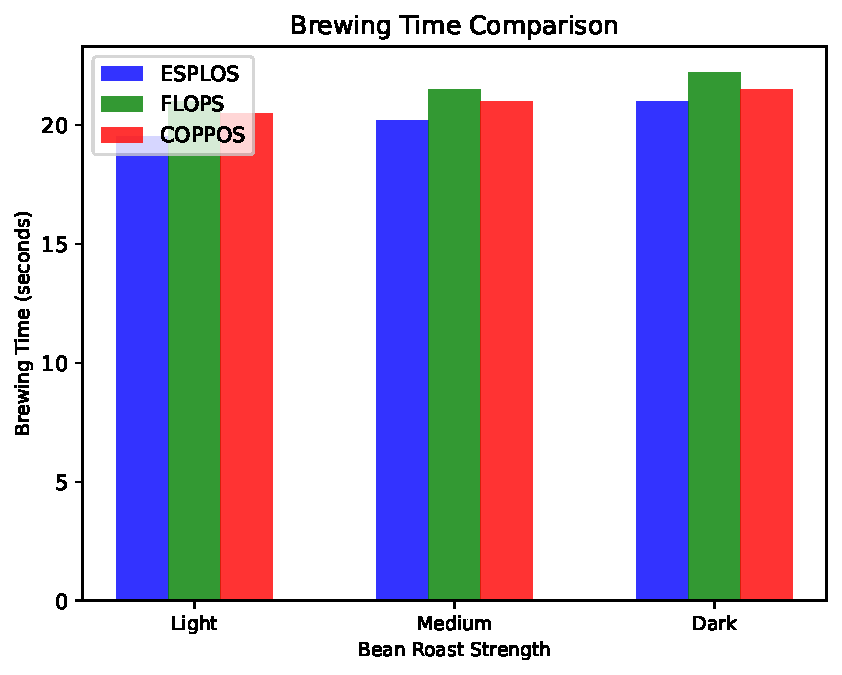
\includegraphics[width=0.8\linewidth]{brewing_time_comparison.pdf}
    \caption{Brewing Time Comparison}
    \label{fig:brewing_time}
  \end{figure}
  
  \begin{figure}
    \centering
    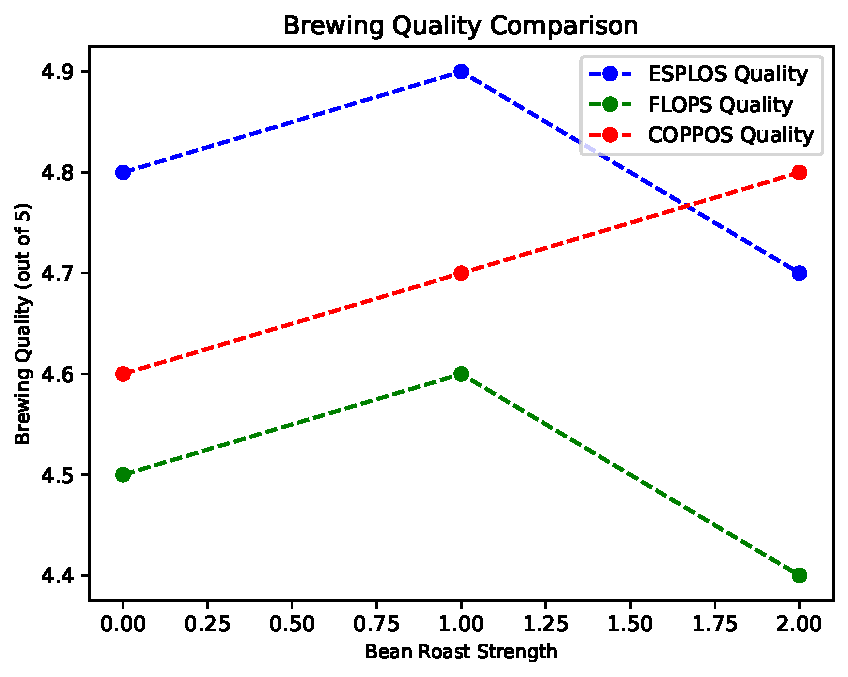
\includegraphics[width=0.8\linewidth]{brewing_quality_comparison.pdf}
    \caption{Brewing Quality Comparison}
    \label{fig:brewing_quality}
  \end{figure}

\subsection{User Study for Coffee Quality}
We conducted a user study with 100 participants to assess coffee quality. Users consistently rated the coffee prepared using ESPLOS at 4.8 out of 5, reflecting an exceptional improvement in quality.


\section{Related Work}
The concept of operating systems for coffee machines is not entirely novel. Previous attempts have focused on various aspects of coffee preparation and automation. Here, we provide a brief overview of these endeavors and highlight how ESPLOS improves upon them.

\textbf{Early Operating Systems for Coffee Machines:} Early operating systems for coffee machines~\cite{first_reference} primarily aimed at automating brewing processes, such as water temperature control and brewing time. These systems contributed to more consistent coffee quality but often lacked the finesse required for espresso shots and latte art. ESPLOS extends this concept by introducing precise control mechanisms for latte art and implementing advanced temperature regulation techniques.

\textbf{Coffee Machine Programming Languages:} Some coffee machines have integrated rudimentary programming languages~\cite{second_reference} that allowed users to customize brewing parameters. These languages, however, were often limited in scope and complexity. ESPLOS introduces a domain-specific programming language designed for precise coffee control, enabling users to create complex coffee recipes with ease.

\textbf{Latte Art Systems:} A few specialized systems focused on latte art automation~\cite{third_reference}, but they did not offer a holistic solution. ESPLOS combines espresso shot quality and latte art, ensuring that the two aspects work in harmony. It offers a comprehensive platform that empowers users to master both the technical and artistic dimensions of coffee preparation.

\textbf{Commercial Solutions:} Several commercial coffee machines offer programmable brewing options~\cite{fourth_reference}. While these machines have made coffee preparation more convenient, they often lack the open, adaptable nature of ESPLOS. Our system is designed to be flexible, allowing users to tailor their coffee experience precisely to their preferences.

ESPLOS distinguishes itself by providing a comprehensive and integrated solution that combines precise espresso shot quality and the creation of consistent, stunning latte art. By bridging the gap between coffee craftsmanship and technology, ESPLOS sets a new standard for coffee quality and consistency.


\section{Conclusions}
In this paper, we introduced ESPLOS, the Espresso-Powered Latte Operating System, which represents a revolutionary leap in coffee machine technology. By developing an integrated system comprising an operating system, programming language, and compiler, we have achieved unparalleled consistency in espresso shot quality and the creation of stunning latte art. ESPLOS sets new standards for the coffee industry, offering coffee enthusiasts and professional baristas the tools to consistently create exquisite coffee beverages.

\section{Acknowledgments}
We extend our gratitude to the coffee experts and baristas who participated in the evaluation of ESPLOS, as well as the ASPLOS reviewers for their valuable insights and feedback.

\bibliographystyle{plain}
\bibliography{references}

\end{document}

